% LaTeX source for ``Introduction to Computer Science (Python Edition)''
% Copyright (c) 2021- David S. Read, All Rights Reserved
% Built upon, ``Python for Informatics: Exploring Information''
% Copyright (c)  2010-  Charles R. Severance, All Rights Reserved

\chapter{Functions}
\label{funcchap}

\section{Function calls}
\label{functionchap}
\index{function call}

In the context of programming, a {\bf function} is a named sequence of
statements that performs a computation.  When you define a function,
you specify the name and the sequence of statements.  Later, you can
``call'' the function by name.  
We have already seen one example of a {\bf function call}:

\beforeverb
\begin{verbatim}
>>> type(32)
<type 'int'>
\end{verbatim}
\afterverb
%
The name of the function is {\tt type}.  The expression in parentheses
is called the {\bf argument} of the function.  The argument is 
a value or variable that we are passing into the function as input 
to the function.  
The result, for the {\tt type} function, is the type of the argument.

\index{parentheses!argument in}

It is common to say that a function ``takes'' an argument and ``returns''
a result.  The result is called the {\bf return value}.

\index{argument}
\index{return value}

\section{Built-in functions}

Python provides a number of important built-in functions that
we can use without needing to provide the function definition.
The creators of Python wrote a set of functions 
to solve common problems and included them in Python for us to use.

The {\tt max} and {\tt min} functions give us the largest and 
smallest values in a list, respectively:

\beforeverb
\begin{verbatim}
>>> max('Hello world')
'w'
>>> min('Hello world')
' '
>>>
\end{verbatim}
\afterverb
%
The {\tt max} function tells us the ``largest character'' in the 
string (which turns out to be the letter ``w'') and the {\tt min}
function shows us the smallest character (which turns out to be a 
space).

Another very common built-in function is the {\tt len} function
which tells us how many items are in its argument. If the argument
to {\tt len} is a string, it returns the number of characters 
in the string.

\beforeverb
\begin{verbatim}
>>> len('Hello world')
11
>>>
\end{verbatim}
\afterverb
%
These functions are not limited to looking at strings. They can operate
on any set of values, as we will see in later chapters.

{\bf You should treat the names of built-in functions as reserved words} (i.e.,
avoid using ``max'' as a variable name). Creating variables whose names match a function will lead to errors when you try to use those functions.

\section{Type conversion functions}
\index{conversion!type}
\index{type conversion}

% from Elkner:
% comment on whether these things are _really_ functions?
% use max as an example of a built-in?

% my reply:
% they are on the list of ``built-in functions'' so I am
% willing to call them functions.

Python also provides built-in functions that convert values
from one type to another.  The {\tt int} function takes any value and
converts it to an integer, if it can, or complains otherwise:

\index{int function}
\index{function!int}

\beforeverb
\begin{verbatim}
>>> int('32')
32
>>> int('Hello')
ValueError: invalid literal for int(): Hello
\end{verbatim}
\afterverb
%
{\tt int} can convert floating-point values to integers, but it
doesn't round off; it chops off the fraction part:

\beforeverb
\begin{verbatim}
>>> int(3.99999)
3
>>> int(-2.3)
-2
\end{verbatim}
\afterverb
%
{\tt float} converts integers and strings to floating-point
numbers:

\index{float function}
\index{function!float}

\beforeverb
\begin{verbatim}
>>> float(32)
32.0
>>> float('3.14159')
3.14159
\end{verbatim}
\afterverb
%
Finally, {\tt str} converts its argument to a string:

\index{str function}
\index{function!str}

\beforeverb
\begin{verbatim}
>>> str(32)
'32'
>>> str(3.14159)
'3.14159'
\end{verbatim}
\afterverb
%

\section{Random numbers}

\index{random number}
\index{number, random}
\index{deterministic}
\index{pseudorandom}

Given the same inputs, most computer programs generate the same
outputs every time, so they are said to be {\bf deterministic}.
Determinism is usually a good thing, since we expect the same
calculation to yield the same result.  For some applications, though,
we want the computer to be unpredictable.  Games are an obvious
example, but there are more.

Making a program truly nondeterministic turns out to be not so easy,
but there are ways to make it at least seem nondeterministic.  One of
them is to use {\bf algorithms} that generate {\bf pseudorandom} numbers.
Pseudorandom numbers are not truly random because they are generated
by a deterministic computation, but just by looking at the numbers it
is all but impossible to distinguish them from random.

\index{random module}
\index{module!random}

The {\tt random} module provides functions that generate
pseudorandom numbers (which I will simply call ``random'' from
here on).

\index{random function}
\index{function!random}

The function {\tt random} returns a random float
between 0.0 and 1.0 (including 0.0 but not 1.0).  Each time you
call {\tt random}, you get the next number in a long series.  To see a
sample, run this loop:

\beforeverb
\begin{verbatim}
import random

for i in range(10):
    x = random.random()
    print x
\end{verbatim}
\afterverb
%
This program produces the following list of 10 random numbers
between 0.0 and up to but not including 1.0.

\beforeverb
\begin{verbatim}
0.301927091705
0.513787075867
0.319470430881
0.285145917252
0.839069045123
0.322027080731
0.550722110248
0.366591677812
0.396981483964
0.838116437404
\end{verbatim}
\afterverb
%
\begin{ex}
Run the program on your system and see what numbers you get.
Run the program more than once and see what numbers you get.
\end{ex}

The {\tt random} function is only one of many 
functions that handle random numbers.
The function {\tt randint} takes the parameters {\tt low} and
{\tt high}, and returns an integer between {\tt low} and
{\tt high} (including both).

\index{randint function}
\index{function!randint}

\beforeverb
\begin{verbatim}
>>> random.randint(5, 10)
5
>>> random.randint(5, 10)
9
\end{verbatim}
\afterverb
%
To choose an element from a sequence\footnote{We'll cover sequences in a future chapter} at random, you can use
{\tt choice}:

\index{choice function}
\index{function!choice}

\beforeverb
\begin{verbatim}
>>> t = [1, 2, 3]
>>> random.choice(t)
2
>>> random.choice(t)
3
\end{verbatim}
\afterverb
%
The {\tt random} module also provides functions to generate
random values from continuous distributions including
Gaussian, exponential, gamma, and a few more.

\section{Math functions}
\index{math function}
\index{function, math}
\index{module}
\index{module object}

Python has a {\tt math} module that provides most of the familiar
mathematical functions.  
Before we can use the module, we have to import it:

\beforeverb
\begin{verbatim}
>>> import math
\end{verbatim}
\afterverb
%
This statement creates a {\bf module object} named math.  If
you print the module object, you get some information about it:

\beforeverb
\begin{verbatim}
>>> print math
<module 'math' from '/usr/lib/python2.5/lib-dynload/math.so'>
\end{verbatim}
\afterverb
%
The module object contains the functions and variables defined in the
module\footnote{We'll learn how to create our own modules later in the course}.  To access one of the functions, you have to specify the name
of the module and the name of the function, separated by a dot (also
known as a period).  This format is called {\bf dot notation}.

\index{dot notation}

\beforeverb
\begin{verbatim}
>>> ratio = signal_power / noise_power
>>> decibels = 10 * math.log10(ratio)

>>> radians = 0.7
>>> height = math.sin(radians)
\end{verbatim}
\afterverb
%
The first example computes the logarithm base 10 of the
signal-to-noise ratio.  The math module also provides a
function called {\tt log} that computes logarithms base {\tt e}.

\index{log function}
\index{function!log}
\index{sine function}
\index{radian}
\index{trigonometric function}
\index{function, trigonometric}

The second example finds the sine of {\tt radians}.  The name of the
variable is a hint that {\tt sin} and the other trigonometric
functions ({\tt cos}, {\tt tan}, etc.)  take arguments in radians. To
convert from degrees to radians, divide by 360 and multiply by $2
\pi$:

\beforeverb
\begin{verbatim}
>>> degrees = 45
>>> radians = degrees / 360.0 * 2 * math.pi
>>> math.sin(radians)
0.707106781187
\end{verbatim}
\afterverb
%
The expression {\tt math.pi} gets the variable {\tt pi} from the math
module.  The value of this variable is an approximation
of $\pi$, accurate to about 15 digits.

\index{pi}

If you know
your trigonometry, you can check the previous result by comparing it to
the square root of two divided by two:

\index{sqrt function}
\index{function!sqrt}

\beforeverb
\begin{verbatim}
>>> math.sqrt(2) / 2.0
0.707106781187
\end{verbatim}
\afterverb
%


\section{Creating functions}

So far, we have only been using the functions that come with Python,
but it is also possible to create our own functions. This allows us to add new functions beyond those provided by Python.

A {\bf function definition} specifies the name of a new function and
the sequence of statements that execute when the function is called.
Once we define a function, we can reuse the function over and over 
throughout our program.

\index{function}
\index{function definition}
\index{definition!function}

Here is an example:

\beforeverb
\begin{verbatim}
def print_lyrics():
    print("I'm a lumberjack, and I'm okay.")
    print('I sleep all night and I work all day.')
\end{verbatim}
\afterverb
%
{\tt def} is a keyword that indicates that this is a function
definition.  The name of the function is \verb"print_lyrics".  The
rules for function names are the same as for variable names: letters,
numbers and some punctuation marks are legal, but the first character
can't be a number.  You can't use a keyword as the name of a function,
and you should avoid having a variable and a function with the same
name.

\index{def keyword}
\index{keyword!def}
\index{argument}

The empty parentheses after the name indicate that this function
doesn't take any arguments.   Later we will build functions that 
take arguments as their inputs.

\index{parentheses!empty}
\index{header}
\index{body}
\index{indentation}
\index{colon}

The first line of the function definition is called the {\bf header};
the rest is called the {\bf body}.  The header has to end with a colon
and the body has to be indented.  By convention, the indentation is
always four spaces.  The body can contain
any number of statements.

The strings in the print statements are enclosed in
quotes.  Single quotes and double quotes do the same thing;
most people use single quotes except in cases like this where
a single quote (which is also an apostrophe) appears in the string.

\index{ellipses}

If you type a function definition in interactive mode, the interpreter
prints ellipses (\emph{...}) to let you know that the definition
isn't complete:

\beforeverb
\begin{verbatim}
>>> def print_lyrics():
...     print("I'm a lumberjack, and I'm okay.")
...     print('I sleep all night and I work all day.')
...
\end{verbatim}
\afterverb
%
To end the function, you have to enter an empty line (this is
not necessary in a script).

Defining a function creates a variable with the same name.

\beforeverb
\begin{verbatim}
>>> print(print_lyrics)
<function print_lyrics at 0xb7e99e9c>
>>> print(type(print_lyrics))
<type 'function'>
\end{verbatim}
\afterverb
%
The value of \verb"print_lyrics" is a {\bf function object}, which
has type \verb"'function'".

\index{function object}
\index{object!function}

The syntax for calling the new function is the same as
for built-in functions:

\beforeverb
\begin{verbatim}
>>> print_lyrics()
I'm a lumberjack, and I'm okay.
I sleep all night and I work all day.
\end{verbatim}
\afterverb
%
Once you have defined a function, you can use it inside another
function.  For example, to repeat the previous refrain, we could write
a function called \verb"repeat_lyrics":

\beforeverb
\begin{verbatim}
def repeat_lyrics():
    print_lyrics()
    print_lyrics()
\end{verbatim}
\afterverb
%
And then call \verb"repeat_lyrics":

\beforeverb
\begin{verbatim}
>>> repeat_lyrics()
I'm a lumberjack, and I'm okay.
I sleep all night and I work all day.
I'm a lumberjack, and I'm okay.
I sleep all night and I work all day.
\end{verbatim}
\afterverb
%
But that's not really how the song goes.


\section{Definitions and uses}
\index{function definition}

Pulling together the code fragments from the previous section, the
whole program looks like this:

\beforeverb
\begin{verbatim}
def print_lyrics():
    print("I'm a lumberjack, and I'm okay.")
    print('I sleep all night and I work all day.')

def repeat_lyrics():
    print_lyrics()
    print_lyrics()

repeat_lyrics()
\end{verbatim}
\afterverb
%
This program contains two function definitions: \verb"print_lyrics" and
\verb"repeat_lyrics".  Function definitions get executed just like other
statements, but the effect is to create function objects.  The statements
inside the function do not get executed until the function is called, and
the function definition generates no output.

\index{use before def}

As you might expect, you have to create a function before you can
execute it.  In other words, the function definition has to be
executed before the first time it is called.

\begin{ex}
Move the last line of this program
to the top, so the function call appears before the definitions. Run 
the program and see what error
message you get.
\end{ex}

\begin{ex}
Move the function call back to the bottom
and move the definition of \verb"print_lyrics" after the definition of
\verb"repeat_lyrics".  What happens when you run this program?
\end{ex}


\section{Flow of execution}
\index{flow of execution}

In order to ensure that a function is defined before its first use,
you have to know the order in which statements are executed, which is
called the {\bf flow of execution}.

Execution always begins at the first statement of the program.
Statements are executed one at a time, in order from top to bottom.

Function \emph{definitions} do not alter the flow of execution of the
program, but remember that statements inside the function are not
executed until the function is called.

A function call is like a detour in the flow of execution. Instead of
going to the next statement, the flow jumps to the body of
the function, executes all the statements there, and then comes back
to pick up where it left off.

That sounds simple enough, until you remember that one function can
call another.  While in the middle of one function, the program might
have to execute the statements in another function. But while
executing that new function, the program might have to execute yet
another function!

Fortunately, Python is good at keeping track of where it is, so each
time a function completes, the program picks up where it left off in
the function that called it.  When it gets to the end of the program,
it terminates.

\begin{minipage}{\textwidth}\label{ch4TraceFlow}
Here is a depiction of a program, traceflow.py, numbering the statements in the order they will execute. The arrows depict the function calls which cause the flow of execution to change.

\beforefig
\centerline{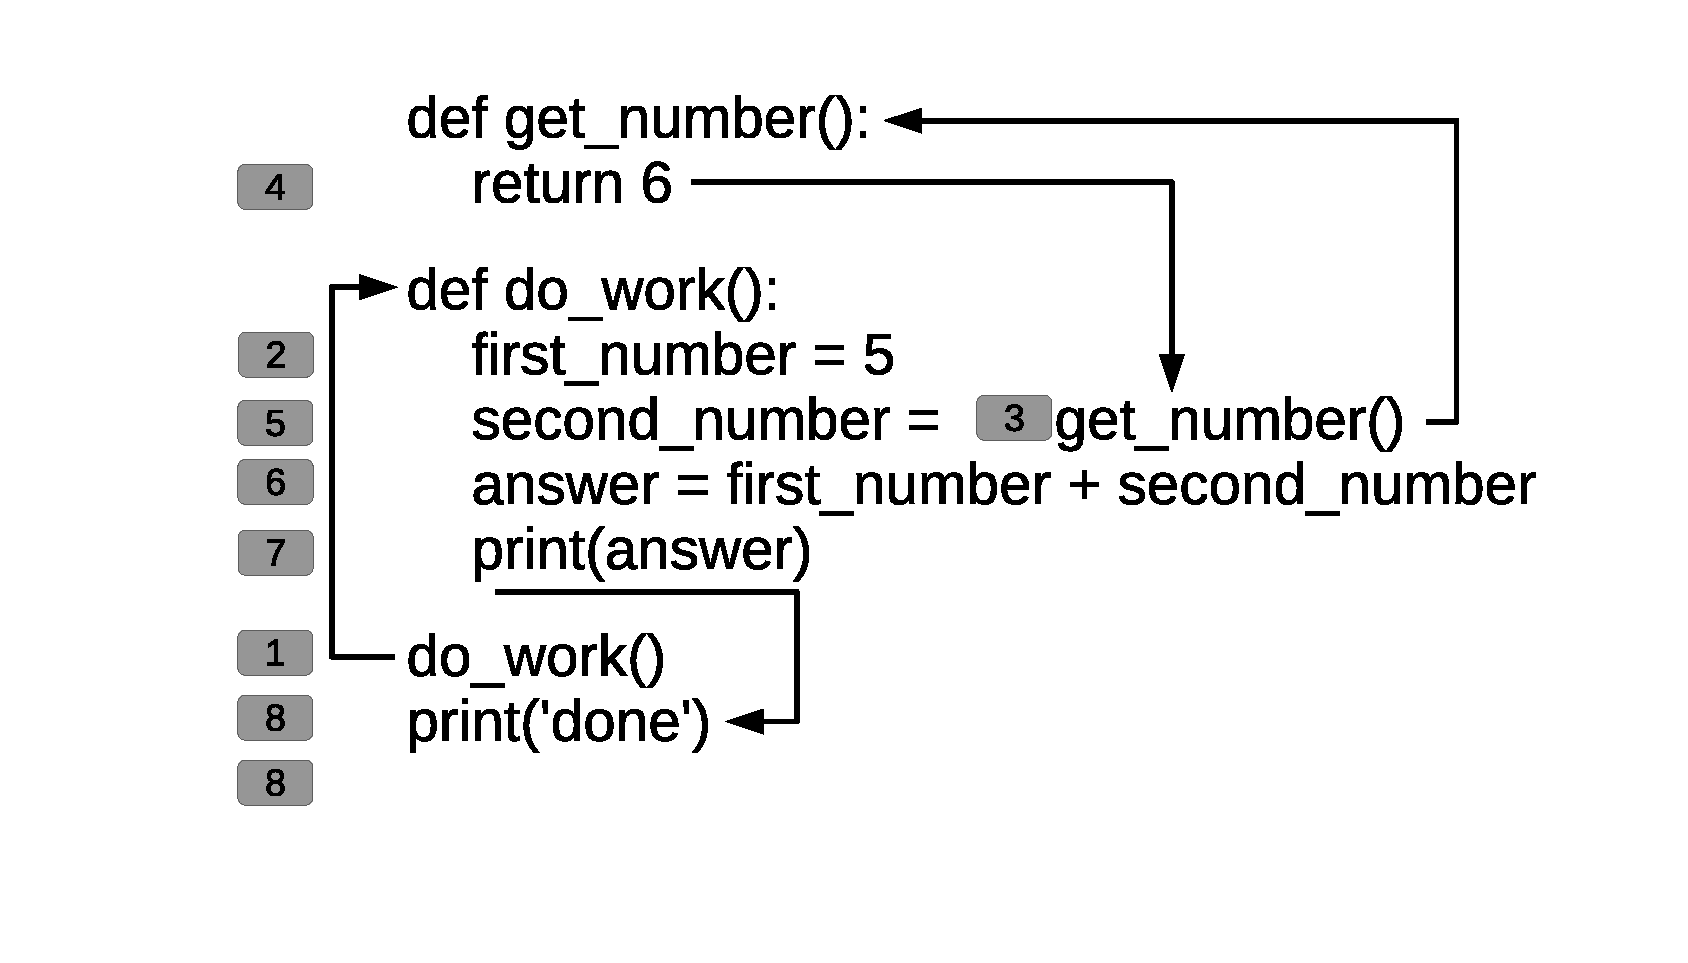
\includegraphics[height=3.5in]{figs2/traceflow.eps}}
\afterfig
\end{minipage}

Running the \texttt{traceflow.py} program would produce this output on the screen:

\beforeverb
\begin{verbatim}
11
done
\end{verbatim}
\afterverb


What's the moral of this sordid tale?  When you read a program, you
don't always want to read from top to bottom.  Sometimes it makes
more sense if you follow the flow of execution.


\section{Parameters and arguments}
\label{parameters}
\index{parameter}
\index{function parameter}
\index{argument}
\index{function argument}

Some of the built-in functions we have seen require arguments.  For
example, when you call {\tt math.sin} you pass a number
as an argument.  Some functions take more than one argument:
{\tt math.pow} takes two, the base and the exponent.

Inside the function, the arguments are assigned to
variables called {\bf parameters}.  Here is an example of a
user-defined function that takes an argument:

\index{parentheses!parameters in}

\beforeverb
\begin{verbatim}
def print_twice(bruce):
    print(bruce)
    print(bruce)
\end{verbatim}
\afterverb
%
This function assigns the argument to a parameter
named {\tt bruce}.  When the function is called, it prints the value of
the parameter (whatever it is) twice.

This function works with any value that can be printed.

\beforeverb
\begin{verbatim}
>>> print_twice('Spam')
Spam
Spam
>>> print_twice(17)
17
17
>>> print_twice(math.pi)
3.14159265359
3.14159265359
\end{verbatim}
\afterverb
%
The same rules of composition that apply to built-in functions also
apply to user-defined functions, so we can use any kind of expression
as an argument for \verb"print_twice":

\index{composition}

\beforeverb
\begin{verbatim}
>>> print_twice('Spam '*4)
Spam Spam Spam Spam
Spam Spam Spam Spam
>>> print_twice(math.cos(math.pi))
-1.0
-1.0
\end{verbatim}
\afterverb
%
The argument is evaluated before the function is called, so
in the examples the expressions \verb"'Spam '*4" and
{\tt math.cos(math.pi)} are only evaluated once.

\index{argument}

You can also use a variable as an argument:

\beforeverb
\begin{verbatim}
>>> michael = 'Eric, the half a bee.'
>>> print_twice(michael)
Eric, the half a bee.
Eric, the half a bee.
\end{verbatim}
\afterverb
%
The name of the variable we pass as an argument ({\tt michael}) has
nothing to do with the name of the parameter ({\tt bruce}).  It
doesn't matter what the value was called back home (in the caller);
here in \verb"print_twice", we call everybody {\tt bruce}.

\section{Fruitful functions and void functions}

\index{fruitful function}
\index{void function}
\index{function, fruitful}
\index{function, void} 

Some of the functions we are using, such as the math functions, yield
results; for lack of a better name, I call them {\bf fruitful
  functions}.  Other functions, like \verb"print_twice", perform an
action but don't return a value.  They are called {\bf void
  functions}.

When you call a fruitful function, you almost always
want to do something with the result; for example, you might
assign it to a variable or use it as part of an expression:

\beforeverb
\begin{verbatim}
x = math.cos(radians)
golden = (math.sqrt(5) + 1) / 2
\end{verbatim}
\afterverb
%
When you call a function in interactive mode, Python displays
the result:

\beforeverb
\begin{verbatim}
>>> math.sqrt(5)
2.2360679774997898
\end{verbatim}
\afterverb
%
But in a script, {\bf if you call a fruitful function and do 
not store the result of the function in a variable,
the return value vanishes into the mist!}

\beforeverb
\begin{verbatim}
math.sqrt(5)
\end{verbatim}
\afterverb
%
This script computes the square root of 5, but since it doesn't store
the result in a variable or display the result, it is not very useful.

\index{interactive mode}
\index{script mode}

Void functions might display something on the screen or have some
other effect, but they don't have a return value.  If you try to
assign the result to a variable, you get a special value called
{\tt None}.

\index{None special value}
\index{special value!None}

\beforeverb
\begin{verbatim}
>>> result = print_twice('Bing')
Bing
Bing
>>> print result
None
\end{verbatim}
\afterverb
%
The value {\tt None} is not the same as the string \verb"'None'". 
It is a special value that has its own type:

\beforeverb
\begin{verbatim}
>>> print type(None)
<type 'NoneType'>
\end{verbatim}
\afterverb
%
To return a result from a function, we use the {\tt return} statement 
in our function.  For example, we could make a very 
simple function called {\tt addtwo}
that adds two numbers together and returns a result.

\beforeverb
\begin{verbatim}
def addtwo(a, b):
    added = a + b
    return added

x = addtwo(3, 5)
print(x)
\end{verbatim}
\afterverb
%
When this script executes, the {\tt print} statement will print out ``8''
because the {\tt addtwo} function was called with 3 and 5 as arguments.
Within the function, the parameters {\tt a} and {\tt b} were 3 and 5 
respectively. The function computed the sum of the two numbers and placed
it in the local function variable named {\tt added}. 
Then it used the {\tt return} statement 
to send the computed value back to the calling code 
as the function result, which was assigned
to the variable {\tt x} and printed out.


\section{Why functions?}
\index{function, reasons for}

It may not be clear why it is worth the trouble to divide
a program into functions.  There are several reasons:

\begin{itemize}

\item Creating a new function gives you an opportunity to name a group
of statements, which makes your program easier to read, understand, 
and debug.

\item Functions can make a program smaller by eliminating repetitive
code.  Later, if you make a change, you only have
to make it in one place.

\item Dividing a long program into functions allows you to debug the
parts one at a time and then assemble them into a working whole.

\item Well-designed functions are often useful for many programs.
Once you write and debug one, you can reuse it.

\end{itemize}

Throughout the rest of the book, often we will use a function definition to 
explain a concept.  Part of the skill of creating and using functions is
to have a function properly capture an idea such as ``find the smallest
value in a list of values''.  Later we will show you code that finds
the smallest in a list of values and we will present it to you as a function
named {\tt min} which takes a list of values as its argument and 
returns the smallest value in the list.


\section{Debugging}
\label{editor}
\index{debugging}

If you are using a text editor to write your scripts, you might
run into problems with spaces and tabs.  The best way to avoid
these problems is to use spaces exclusively (no tabs).  Most text
editors that know about Python do this by default, but some
don't.

\index{whitespace}

Tabs and spaces are usually invisible, which makes them
hard to debug, so try to find an editor that manages indentation
for you.

Also, don't forget to save your program before you run it.  Some
development environments do this automatically, but some don't.
In that case, the program you are looking at in the text editor
is not the same as the program you are running.

Debugging can take a long time if you keep running the same
incorrect program over and over!

Make sure that the code you are looking at is the code you are running.
If you're not sure, put something like \verb"print('hello')" at the
beginning of the program and run it again.  If you don't see
\verb"hello", you're not running the right program!




\section{Glossary}

\begin{description}

\item[algorithm:]  A general process for solving a category of
problems.
\index{algorithm}

\item[argument:]  A value provided to a function when the function is called.
This value is assigned to the corresponding parameter in the function.
\index{argument}

\item[body:] The sequence of statements inside a function definition.
\index{body}

\item[composition:] Using an expression as part of a larger expression,
or a statement as part of a larger statement.
\index{composition}

\item[deterministic:] Pertaining to a program that does the same
thing each time it runs, given the same inputs.
\index{deterministic}

\item[dot notation:]  The syntax for calling a function in another
module by specifying the module name followed by a dot (period) and
the function name.
\index{dot notation}

\item[flow of execution:]  The order in which statements are executed during
a program run.
\index{flow of execution}

\item[fruitful function:] A function that returns a value.
\index{fruitful function}

\item[function:] A named sequence of statements that performs some
useful operation.  Functions may or may not take arguments and may or
may not produce a result.
\index{function}

\item[function call:] A statement that executes a function. It
consists of the function name followed by an argument list.
\index{function call}

\item[function definition:]  A statement that creates a new function,
specifying its name, parameters, and the statements it executes.
\index{function definition}

\item[function object:]  A value created by a function definition.
The name of the function is a variable that refers to a function
object.
\index{function definition}

\item[header:] The first line of a function definition.
\index{header}

\item[import statement:] A statement that reads a module file and creates
a module object.
\index{import statement}
\index{statement!import}

\item[module object:] A value created by an {\tt import} statement
that provides access to the data and code defined in a module.
\index{module}

\item[parameter:] A name used inside a function to refer to the value
passed as an argument.
\index{parameter}

\item[pseudorandom:] Pertaining to a sequence of numbers that appear
to be random, but are generated by a deterministic program.
\index{pseudorandom}

\item[return value:]  The result of a function.  If a function call
is used as an expression, the return value is the value of
the expression.
\index{return value}

\item[void function:] A function that does not return a value.
\index{void function}


\end{description}


\section{Exercises}

\begin{ex}
What is the purpose of the "def" keyword in Python?

a) It is slang that means "the following code is really cool"\\
b) It indicates the start of a function\\
c) It indicates that the following indented section of code is to be stored for later\\
d) b and c are both true\\
e) None of the above
\end{ex}

\begin{ex}
What will the following Python program print out?

\beforeverb
\begin{verbatim}
def fred():
   print("Zap")

def jane():
   print("ABC")

jane()
fred()
jane()
\end{verbatim}
\afterverb
%
a) Zap ABC jane fred jane\\
b) Zap ABC Zap\\
c) ABC Zap jane\\
d) ABC Zap ABC\\
e) Zap Zap Zap
\end{ex}

\begin{ex}
Rewrite your pay computation (exercise \ref{exCh3HourRate}, page \pageref{exCh3HourRate}) with time-and-a-half for overtime
and create a function called {\tt computepay} which takes
two parameters ({\tt hours} and {\tt rate}).

\begin{verbatim}
Enter Hours: 45
Enter Rate: 10
Pay: 475.0
\end{verbatim}
\end{ex}

\begin{ex}
Rewrite the grade program (exercise \ref{exCh3Score}, page \pageref{exCh3Score})
using a function called {\tt computegrade} that takes
a score as its parameter and returns a grade as a string.

\begin{verbatim}
Score   Grade
> 0.9     A
> 0.8     B
> 0.7     C
> 0.6     D
<= 0.6    F

Program Execution:

Enter score: 0.95
A

Enter score: perfect
Bad score

Enter score: 10.0
Bad score

Enter score: 0.75
C

Enter score: 0.5
F
\end{verbatim}

Run the program repeatedly to test the various different values
for input.
\end{ex}
\begin{ex}
Retype the traceflow program (page \pageref{ch4TraceFlow}) into a file on your computer called traceflow.py and run it. Verify you get the expected results. 

Next, modify the {\tt def\_number()} function to accept a number from the user (use the {\tt input()} function) and return the value entered by the user. Test your updated program and verify the new output is what you expect.
\end{ex}